\xchapter{Fundamentação}{Serão apresentadas as principais referências teóricas que reunidas constituem uma base para a elaboração do trabalho.}

\acresetall 

\section{Simulação baseada em física}

O processo da impressão hidrográfica é um fenômeno físico que envolve a interação entre dois objetos principais: um deles é a superfície 3D que está sendo pintada, o outro é o filme 2D que carrega a imagem impressa. O filme permanece flutuando na superfície da água, formando um composto imiscível. Comporta-se como uma lâmina viscosa que ao tocar na superfície do objeto, adere quase que imediatamente à superfície deste objeto, acompanhando o movimento de imersão. Ao fim da operação, os pontos da imagem impressa no filme ocuparão uma determinada posição no objeto.

A simulação baseada em física é a área de estudo na computação gráfica que busca, através do suporte da física, gerar simulações realistas de fenômenos naturais. Os principais avanços nesta área foram motivados pela necessidade de uma representação virtual consistente das interações complexas entre corpos. Estes estudos possibilitaram incrementar os efeitos especiais na indústria cinematográfica, assim como na indústria de entretenimento com jogos \cite{reeves1983particle} \cite{millington2007game}.

No design de produtos e sobretudo na engenharia, a simulação com computação gráfica tem sido particularmente útil no sentido de prever o comportamento de sistemas físicos complexos, sem a necessidade de um experimento real, economizando-se o tempo, a mão de obra e o material que seria empenhado. A figura \ref{fig:pipeline1} ilustra esta idéia, representando as etapas que vão desde a simulação da pintura hidrográfica até a realização da pintura física do objeto.

\begin{figure}
\begin{center} 
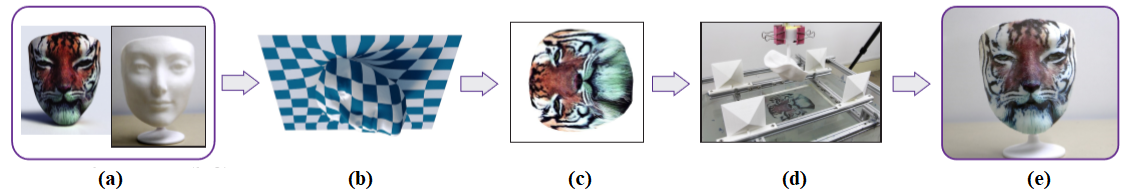
\includegraphics[scale=0.5]{pipeline.png}
\caption{Representação dos passos desde a simulação da pintura hidrográfica até a pintura física do objeto. \textbf{(a)} Textura (à esquerda) e objeto (à direita). \textbf{(b)} Simulação. \textbf{(c)} Filme gerado com base na simulação. \textbf{(e)} Pintura hidrográfica física. \textbf{(f)} Resultado final do objeto 3D colorido com pintura hidrográfica. \cite{zhang2015}.}
\label{fig:pipeline1}
\end{center} 
\end{figure}

Simulações podem ser \textit{offline}, quando o usuário não interage com os elementos da cena. Isto ocorre na indústria cinematográfica, pois os quadros da animação são produzidos anteriormente, durante a criação do filme. No caso de jogos, ou de aplicações que demandem uma interação com o usuário, será necessário realizar a simulação em tempo real. Para os padrões modernos, a apresentação de uma animação exibida em taxas acima de 25 \acs{FPS} (\acl{FPS}) já pode ser considerada em tempo real.

O problema da simulação baseada em física traz encadeado o problema da detecção de colisão como uma etapa importante. Neste ponto, existem técnicas documentadas que dão o tratamento adequado para detectar a colisão entre os corpos, impondo ao sistema restrições importantes quanto a movimentação destes corpos. \cite{moore1988collision} \cite{jimenez20013d}

Dentre os estudos desenvolvidos, simulações baseadas em física podem ser classificadas em diversas categorias, cada uma com características próprias e um conjunto de problemas técnicos a serem resolvidos. Destacam-se então: a simulação de corpos rígidos, simulação de corpos deformáveis, simulação de partículas, simulação de multidões e a simulação de fluidos. 

Para o desenvolvimento deste projeto, após uma análise do que ocorre no experimento físico conforme \ref{apendice1:etapas}, foi considerado que a modelagem simulação levaria principalmente à condição de um fenômeno de interação entre um corpo deformável (o filme com a película hidrográfica) e um corpo rígido movimentado com velocidade constante (o objeto que será pintado). Apesar de existir a interação do objeto e do filme com um fluido (a água), observou-se que idealmente o sistema formado não deve sofrer interferência significativa da água, pois a película permanece na superfície sem se misturar com a água.

\subsection{Integração numérica de Euler}

Trata-se do método mais básico de solucionar numericamente equações diferenciais. A proposta de Euler é resolver as equações referentes ao fenômeno estudado com base em integração numérica, atribuindo valores às variáveis e discretizando os valores da função em intervalos conhecidos. Em \cite{baraffphysically} pode ser encontrado um estudo prático no qual são apresentadas aplicações do método de Euler em simulações computacionais.

Por tratar-se de uma discretização de valores contínuos, no método de Euler será necessário determinar arbitrariamente o valor do intervalo utilizado, de forma que produza valores consistentes com o que se deseja implementar. Um intervalo muito grande, produzirá erros maiores. Um intervalo muito pequeno, produzirá aproximações indesejáveis. Para os fenômenos físicos estudados na computação gráfica, o objetivo final será o cálculo da posição dos objetos na cena em função do tempo. 

\subsection{Simulação de corpos deformáveis}

Corpos deformáveis, diferentemente dos corpos rígidos, quando submetidos a forças externas, podem variar a sua forma em uma simulação. A simulação de corpos deformáveis pode representar visualmente o processo que ocorre em uma variedade de materiais como: borracha, plástico, cabelo, músculos, tecidos. Usualmente, neste tipo de simulação, a representação do material se dá através de uma malha contendo massas e molas. Nesta malha, podem ser atribuídas massas aos vértices, enquanto nas arestas são atribuídas molas. A simulação consiste então em calcular as forças de atração e repulsão exercidas entre os pontos do sistema ao longo do tempo. A resistência à deformação de um corpo, por exemplo, será dada pela resistência atribuída às molas que compõem a estrutura deste modelo. Representações 2D deste sistemas apresentarão topologias mais simples de molas. Este \textit{design} está ilustrado na figura \ref{fig:mass-spring}.

\begin{figure}
\begin{center} 
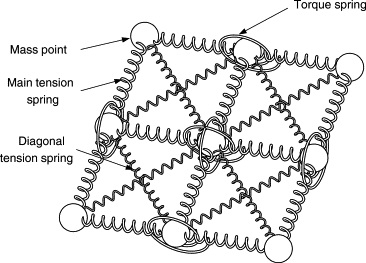
\includegraphics[scale=0.6]{mass-spring.jpg}
\caption{Modelagem de um corpo deformável como um sistema de massas e molas. \cite{gao2006haptic}}
\label{fig:mass-spring}
\end{center} 
\end{figure}

Em \cite{Batty2012}, é apresentado um modelo discreto que representa a dinâmica de fluidos que se apresentem como uma lâmina viscosa, com a preservação do volume. Neste trabalho, a lâmina viscosa é apresentada como um corpo líquido sem forma delimitada, com volume constante, com um grau de elasticidade, uma tensão de superfície e que pode eventualmente interagir com outros corpos rígidos. A proposta modela as lâminas viscosas como malhas de triângulos, que representam o líquido em questão. Com este modelo é possível executar uma simulação discretizada, porém ainda consistente com a física, das forças envolvidas neste tipo de sistema. Uma variedade de líquidos que dobram ou que se enrolam quando derramados (mel, glace, lava) podem ser simulados com base neste trabalho.

\section{\acs{PBD} (\acl{PBD})}

Muitos problemas de simulação física de corpos deformáveis têm sido resolvidos através de métodos matemáticos bem estabelecidos como \acs{MEF} (\acl{MEF}) \cite{jimenez20013d}. Esta técnica possibilita um cálculo com maior exatidão dos valores, contudo leva a um tempo maior de processamento. Por este motivo, simulações em tempo real podem ser inviabilizadas se forem realizadas com \acs{MEF}.

Simulações baseadas em física tradicionalmente tomam como ponto de partida as leis do movimento descritas por Newton, compondo um sistema de forças. O inconveniente deste tipo de simulação é a necessidade de se calcular primeiramente a aceleração das forças envolvidas, para derivar a equação das velocidades envolvidas (primeira ordem) e só então derivar as equações das posições envolvidas (segunda ordem).

No trabalho de \cite{muller2007position} é apresentada a técnica de \acs{PBD}, um tratamento diferente para se modelar uma simulação física. O sistema de forças (tradicional na simulação com base das leis de Newton) fica em segundo plano nesta abordagem. O algoritmo que implementa esta técnica é apresentado na figura \ref{fig:algoritmo_PBD}.

\begin{figure}
\begin{center}
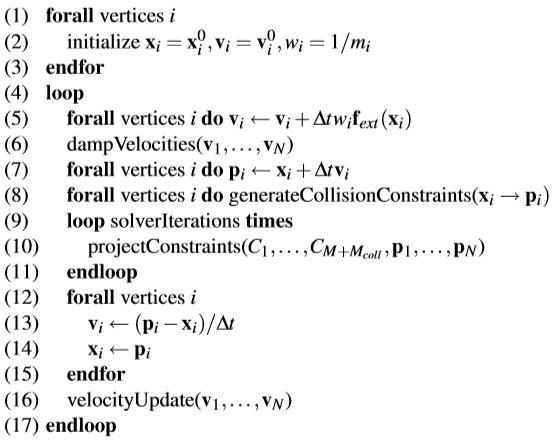
\includegraphics[scale=0.72]{algoritmo_pbd.png}
\caption{Algoritmo \ac{PBD} \cite{muller2007position}}
\label{fig:algoritmo_PBD}
\end{center} 
\end{figure}

Usando \acs{PBD}, os objetos simulados são representados en um conjunto de \textit{N} vértices e \textit{M} restrições. Cada vértice $i \in [1..N]$ possui como atributos importantes a sua posição $x_i$, uma velocidade $v_i$ e uma massa $m_i$. No algoritmo, as linhas (1) a (3) apenas iniciam os valores destes atributos.

Em cada iteração do laço principal do algoritmo linhas (4) até (17), é utilizado o intervalo de tempo $\Delta t$ conforme o método de Euler. A parte que mais diferencia o algoritmo do método de integração de Euler está nas linhas (7), (9) até (11), (13) até (14).

Na linha (7), é calculada uma posição prevista $p_i$ de cada vértice usando uma integração explícita de Euler. Na linha (8), a função \textit{generateCollisionConstraints} realiza a verificação dos vértices que sofreram colisão com outro corpo na simulação. Como resultado desta verificação, um conjunto de restrições de colisão com cardinalidade $M_{col}$ é gerado dinamicamente em cada $\Delta t$. As colisões encontradas nesta verificação são adicionadas ao conjunto original de restrições, ampliando este conjunto para $j \in [1, 2, ...., M, M+1, M+2, ...., M+M_{col}]$. A simulação processará então este novo conjunto de restrições.

Nas linhas (9) até (11), as restrições dos vértices são aplicadas através da solução iterativa para satisfazer o posicionamento de $N$ vértices a $M+M_{col}$ restrições. A quantidade de iterações determinada em $solverIteraction$ é arbitrária, e determinará a dinâmica de correção aplicada à posição prévia $p_i$.
A linha (9) executa a correção propriamente dita da posição $p_i$. Cada restrição $C_j$ está vinculada a um conjunto de vértices. Pode ocorrer de um mesmo vértice estar presente em mais de uma restrição. Como exemplo, uma restrição de distância $d$ entre dois pontos $x_1$ e $x_2$ no espaço ${\rm I\!R}^3$ pode ser formulada como: $C_j(x_1, x_2) = |x_1 - x_2|^2 - d^2$. Satisfazer a esta restrição levará à solução de uma equação não linear. A resolução do conjunto de restrições ${C_1, C_2, ..., C_{Mcol}}$ será feita através de da aproximação para um conjunto de sistemas lineares, conforme as equações adotadas em \cite{muller2007position} que utiliza uma adaptação similar ao método iterativo de Gauss-Siedel. Nos passos (13) e (14), os valores finais das posições são finalmente definidos após a correção. As velocidades decorrentes destes ajustes também são atualizadas.

O algoritmo proposto possui uma estrutura similar com o algoritmo de integração numérica de Euler. Além disso, evita a instabilidade gerada no sistema por conta do uso das equações do movimento de Newton, que necessitam de derivações até a segunda ordem para finalmente determinar as posições dos corpos da cena. Isto porque os passos (13) até (14) não permitem extrapolações da posição prevista $p_i$. Tais extrapolações levariam o cálculo a uma condição impossível do sistema, visto que nos passos anteriores (9) a (11) as posições já foram computadas dentro das restrições permitidas. Por fim, oferece uma alternativa menos custosa que o \acs{MEF} para simular corpos deformáveis, corpos rígidos e fluidos, dentre outros sistemas considerados complexos.

O trabalho de \cite{muller2007position} foi complementado posteriormente na proposta explicada em \cite{fratarcangeli2013gpu}, que oferece uma solução para paralelizar o algoritmo de \ac{PBD}. A proposta leva a uma redução do uso da \acs{CPU} (\acl{CPU}) e a distribuição do processamento para os vários núcleos disponíveis na \acs{GPU} (\acl{GPU}). Isto deixa a execução da animação sem interrupções e favorece a implementação simulações complexas com \acs{PBD} em tempo real.

Outra complementação importante para a técnica \acs{PBD} foi feita mais tarde por \cite{macklin2016xpbd}, que propuseram um método simples para tornar a rigidez dos corpos independente do intervalo de tempo determinado na simulação e independente da quantidade de iterações determinada para resolução das restrições. Com isto, o aspecto visual de elasticidade dos corpos em uma cena torna-se mais controlável através de um parâmetro independente, específico para este fim.

Por fim, a implementação da técnica \ac{PBD} traz uma simplificação para o problema da simulação de corpos deformáveis. As restrições atuarão como uma parametrização do movimento do corpo. A implementação será a resolução numérica de um sistema não linear de equações através de N iterações.

\section{OpenGL}

\subsection{Características}

\acs{OpenGL} (\acl{OpenGL}) é uma \acs{API} (\acl{API}) padrão para a criação de aplicações 3D que precisem apresentar gráficos de qualidade, utilizando os recursos da placa gráfica com eficiência.

O desenvolvimento de software utilizando \acs{OpenGL} permite o acesso aos recursos da placa gráfica, através de um \textit{pipeline} que possui estágios pré-programados e estágios programáveis através da criação de programas denominados \textit{shaders}. O uso do \acs{OpenGL} dá ao usuário o acesso indireto aos recursos de processamento/entrada e saída do dispositivo gráfico através de uma máquina de estados, na qual se inicializam valores em áreas de memória (\textit{buffers}) e submetem estes valores ao comando desejado.

A programação com \acs{OpenGL} exige, portanto, que um passo a passo seja seguido rigorosamente, para que a máquina de estados se mantenha consistente. Cada comando executado levará a máquina a um novo estado e assim por diante. A renderização de uma imagem passa por passos específicos para a criação dos espaços de memória, movimentação dos dados para este espaço, montagem dos dados para desenho, desenho da figura na tela.

\subsection{Programação na GPU com \textit{shaders}}

Na programação com \acs{OpenGL}, a CPU tem como papel de gerenciar informações de entrada/saída, bem como controlar os dados de controle da aplicação principal. A biblioteca \acs{OpenGL} oferece a possibilidade de executar programas na \acs{GPU}, denominados \textit{shaders}. Uma \acs{GPU} é capaz de executar centenas de instruções em paralelo, o que é importante em aplicações gráficas, que frequentemente executam as mesmas instruções para um grande conjunto de dados (pontos) que serão desenhados na tela. A \acs{GPU} poderá acionar diversas instâncias de um mesmo \textit{shader} passando um conjunto de dados diferente. Desta forma, é possível realizar renderizações rapidamente, sem sobrecarregar a CPU. 

A figura \ref{fig:pipeline} representa as etapas programáveis do pipeline do OpenGL. O pipeline inicia com o fornecimento das estruturas de dados que representam as primitivas que serão desenhadas. O conjunto de dados dos vértices são transferidos do programa principal para os \textit{buffers} da \acs{GPU}, iniciando o processamento na etapa do \textit{vertex shader}. Os três passos seguintes são opcionais. As etapas de tesselação cuidam basicamente de possíveis subdivisões das primitivas originais. Caso haja necessidade de modificar a geometria, portanto a primitiva de desenho, então será programado um \textit{shader} específico para a geometria. 

\begin{figure}
\begin{center}
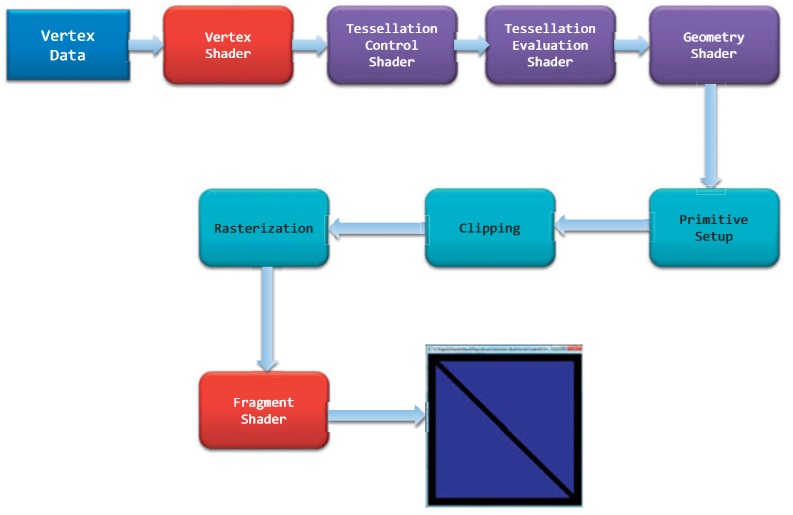
\includegraphics[scale=0.5]{pipeline.jpg}
\caption{Diagrama representativo dos estágios do \ac{OpenGL} \cite{Shreiner:2013:OPG:2544032}}
\label{fig:pipeline}
\end{center} 
\end{figure}

Os \textit{shaders} são programas que operam sobre grandes conjuntos de dados. São especializados de acordo com a etapa do \textit{pipeline} que foram designados. Dentre os \textit{shaders} mais comuns na biblioteca OpenGL, há o \textit{vertex shader} (destinado a operar sobre os vértices do modelo, sendo úteis para o processamento das transformações geométricas), o \textit{fragment shader} (destinado a operar sobre os pixels da imagem gerada, sendo úteis no cálculo e estabelecimento final da cor).

A partir da versão 4.3 do \acs{OpenGL}, é introduzido o \textit{compute shader}. Este tipo de \textit{shader} é particularmente útil quando se deseja realizar processamentos genéricos que não necessariamente irão resultar em dados que se converterão em imagens ou primitivas. Algoritmos paralelizáveis poderão tirar um melhor proveito dos recursos do hardware executando na \acs{GPU} em um \textit{compute shader}. Para simulações baseadas em física, o cálculo necessário para a atualização das velocidades e das posições dos corpos poderão ser paralelizados. Em outro passo, posteriormente, os valores calculados poderão ser transferidos para os \textit{buffers} que serão utilizados pelos vértices que formam a imagem da cena.

Algoritmos de simulação de partículas podem ser paralelizáveis para fornecer uma apresentação fluida, sem interrupções perceptíveis pelo usuário. No caso da simulação de um corpo deformável, a paralelização deverá ser criteriosa, pois há uma interação mútua entre elementos vizinhos pertencentes a uma mesma malha. Neste caso, a atualização concorrente da posição de uma mesma partícula que seja um vizinho em comum causará condições de corrida, provocando uma inconsistência no sistema simulado. 

Uma possível solução para este problema foi estudada em \cite{fratarcangeli2013gpu}. A proposta utiliza o conceito de coloração de grafos para formar grupos de partículas que não tenham um vizinho em comum. Cada partição será processada em paralelo. Como as partições não compartilham partículas, então o problema de inconsistência deixa de existir, e a malha é processada mais rapidamente.

\section{Mapeamento de Texturas}

Mapeamento de texturas é um procedimento bastante utilizado na computação gráfica \cite{haeberli1993texture}. O principal objetivo desta técnica é adicionar realismo a uma cena. A forma mais simples de mapeamento de textura consiste em aplicar uma imagem 2D a um objeto 3D da cena. \cite{shreiner2013opengl}

Para realização desta técnica, define-se uma função de mapeamento entre os domínios 2D (a textura) e 3D (a superfície do modelo) e, em seguida, são criadas coordenadas de textura associadas aos vértices do modelo 3D. Existem diversas maneiras de se definir a função de mapeamento conforme mostrado em \cite{hormann2007mesh}.

Na pintura hidrográfica, o mapeamento da textura será feito em três etapas. 
\begin{itemize}
\item Primeiramente, a superfície textura será aplicada a um plano, modelado como uma malha regular de triângulos, na qual se conhece as posições iniciais de cada ponto da textura neste plano. 
\item Na segunda etapa, executa-se a simulação da impressão hidrográfica e verifica-se como o plano 2D se deformou em relação ao modelo 3D, levando cada ponto do plano 2D de uma posição inicial (antes da deformação do plano) para uma posição final (após a deformação do plano). O mapeamento ocorrerá automaticamente ao se relacionar cada ponto da posição inicial com a posição final. 
\item Por fim, o usuário do sistema, conhecendo como cada região da textura 2D se deformará para encontrar os pontos do objeto impresso em 3D, poderá estabelecer cores arbitrárias para cada região do objeto impresso em 3D. Em seguida, gerará um filme com uma impressão espelhada do  desenho desejado, para finalmente executar a impressão hidrográfica física.
\end{itemize}